\documentclass[12pt]{article}

\usepackage{amsmath}
\usepackage{amssymb}
\usepackage{amsthm}
\usepackage{epsfig}

\newcommand{\XXX}[1]{\textbf{XXX: #1}}

\newtheorem*{Definition}{Definition}
\newtheorem*{Theorem}{Theorem}

\title{Statistical Mechanics and Cellular Automata}
\author{Luke Palmer}

\begin{document}
\maketitle

The theory of cellular automata is one of those fields that has been
around for a decent amount of time (about 40 years), but about which
very little is known.  Minor changes in the rules behind a cellular
automaton usually do not affect its overall qualitiative behavior, but
sometimes they can cause major \textit{bifurcations} in behavior.

Li et al. \cite{Li-1990} explore this idea, and find that with a logical
path through a rule space, there is a transition point between
``simple'' and ``chaotic'' behavior, though it does vary from path to
path.  But near the transition point emerges so-called ``complex''
behavior, which neither looks statistically random nor is periodic.

In this paper, I'll have some fun describing a reasonable precise
definition of a cellular automaton, though I won't use the definitions
for much.  I'll then describe the metrics used by Li et al. and
reproduce some of their graphs with a program I wrote.  

Some slightly domain-specific notation is taken from the theory of
functional programming\footnote{Probably somewhere earlier than that,
actually, but functional programming is the first place I saw it.}.  We
write $f^*(x_1, x_2, ..., x_n)$ to mean $(f(x_1), f(x_2), ..., f(x_n))$.
Similarly, $(x_1, x_2, ..., x_n) +^* k$ means $(x_1 + k, x_2 + k, ...,
x_n + k)$.

\section{Defining Cellular Automata}

A lot of work has been done on cellular automata, but every author has
his own definition of what they are\footnote{And many authors leave the
definition implicit, which is even more problematic when everyone has
his own definition.}.  We wouldn't want to look like a conformist by
copying another author's definition, so here's our own:

\begin{Definition}
An $n$-neighbor cellular topology over a set $C$ is a function $t: C
\mapsto C^n$.  
\end{Definition}

\begin{Definition}
An $n$-neighbor evolver over a set $S$ is a function $e: S^n \mapsto S$.
\end{Definition}

\begin{Definition}
A cellular automaton $A$ is the tuple $(n,C,t,S,e)$ where:
\begin{itemize}
\item $t$ is an $n$-neighbor cellular topology over $C$.
\item $e$ is an $n$-neighbor evolver function over $S$.
\item There exists a $0 \in S$ such that $e(0,0,...) = 0$.
\end{itemize}
We say that $A$ is an $n$-neighbor cellular automaton.  We call $C$ the
set of cells and $S$ the set of states.
\end{Definition}

Notice that there is no connection between $(C,t)$ and $(S,e)$.
Therefore, we can't get any more interesting information studying this
system as a whole than we could by studying these parts.  The
abstraction that connects the two concepts is called a
\textit{configuration}:

\begin{Definition}
A configuration is a function $c: C \mapsto S$.
\end{Definition}

To get something that behaves like what everyone else calls a cellular
automaton, we can derive from an automaton a mapping between
configurations.

\begin{Definition}
The evolution map $E: (C \mapsto S) \mapsto (C \mapsto S)$ of an
automaton is the function $E(c) = e \circ c^* \circ t$.
\end{Definition}

An intuition for the definition of this function is that you give it a
configuration and a cell, and you ask for the state of that cell.  It
does this by looking up the ``predecessors'' of that cell and applying
the evolver to each of their states in the configuration.

Traditionally cellular automata have been defined over a lattice.  We'll
define these over a \textit{linear cellular topology}:

\begin{Definition}
A linear cellular topology is a cellular topology where $(C,+)$ is an
abelian group and $t(k+l) = t(k) +^* l$ for all $k,l \in C$.
\end{Definition}

We call a cellular automaton defined over a linear cellular topology
a \textit{linear cellular automaton}.

\section{Chaos and Complexity}

In studying cellular automata as dynamical systems, we're looking for
chaotic behavior.  Unfortunately, how the literature defines ``chaos''
in a cellular automaton is not analogous to chaos in, say, a continuous
dynamical system.  Chaos in an automaton is approximately when the
system is entirely unpredictable: where each cell in a chaotic region
has an ``equal chance'' of being in any state (which will make more
sense as we switch to a probabilistic view of automata).  This is more
analogous to divergent behavior in a continuous system.  It is also
analogous to the state of highest entropy in a thermodynamic system.

So a better, if more vague, way to state our goal is that we are looking
for ``interesting'' behavior.  Chaotic behavior is not interesting in a
cellular automaton.  Clearly, neither is fixed-point or simple-periodic
(short periods) behavior.  The only remaining kind of behavior is called
``complex behavior'' in the literature.  Supposedly it is defined
precisely as behavior that is neither chaotic nor simple-periodic.

Li et al. define three statistical quantities that are
used for classifying cellular automaton rules.  These are the
\textit{spreading rate of difference patterns}, the \textit{entropy},
and the \textit{mutual information}.  The latter two are repeated here,
since the first one has a complicated definition that is specific to
one-dimensional linear systems and that didn't end up providing very
much useful information.

\begin{Definition}
The entropy $S$ of a probability distribution $p_i$ is defined as:
\[ S = -\sum_i{p_i \log p_i} \]
The summand is defined to be $0$ when $p_i$ is zero.  The resulting
summand is still continuous.
\end{Definition}

One way to calculate the entropy is simply to count all states over
space time.  If this were a two-state system, the sum would only have
two terms.  Another way is to count the states at each time step.  If
the entropy is increasing over time, then that is a good indication of a
chaotic rule.

\begin{Definition}
The mutual information $M$ of a two-variable probability distribution
$p_{ij}$ is defined as
\[ M = \sum_{i,j}{p_{ij} \log \frac{p_{ij}}{p_i p_j}} \]
where $p_i = \sum_j{p_{ij}}$ and $p_j = \sum_i{p_{ij}}$.
\end{Definition}

Intuitively, the entropy defines how distributed the probabilities in
the distribution are.  The entropy takes on its highest value when all
the $p_i$ are equal\footnote{A fact which is apparently non-trivial to
prove.  I tried and failed.  Consider it a challenging exercise for the
reader.}, and it takes on its lowest value when there exactly one
substate with probability $1$ and all others $0$.  The entropy will tell
you how \textit{chaotic}, but not necessarily complex, the system is.

Mutual information is the primary measure of complexity.  Notice that if
the $i$ and $j$ events are uncorrelated, then $p_{ij} = p_i p_j$ and
there will be no contribution to the sum.  It would seem that periodic
motion, which is not complex, would give high values of $M$.  However,
suppose $p_{ij}$ is the probability that cell $a$ has the value $i \in
\{1,2\}$ and cell $b$ has the value $j \in \{1,2\}$.  Also, suppose the
periodic motion is such that they will usually have the same value.
There will be a positive contribution from $p_{11}$ and $p_{22}$.
However, the probability that they are opposite is \textit{lower} than
that of an uncorrelated distribution, so there is a negative
contribution from $p_{12}$ and $p_{21}$, of approximately the same
magnitude.  It looks like $M$ ``rejects'' periodic motion.

\section{Bifurcations in the Rule Space}

We can use these quantities to find bifurcations in the rule space.  Li
et al. \cite{Li-1990} do this for a wide variety of one-dimensional
rules.  I have reproduced their experiment for a smaller class of rules,
namely the one-dimensional binary linear automata on a circle.  

We construct the rules using Wolfram's naming scheme.  For example, for
two-neighbor automata, $\langle 0110 \rangle$ refers to the rule $00
\mapsto 0$, $01 \mapsto 1$, $10 \mapsto 1$, $11 \mapsto 0$.   For the
9-neighbor system shown here, the rules names will be $2^9 = 512$ bits
long.

We compute a path through the 9-neighbor rules as follows.  The first
rule in the path will be all 0s.  The next rule in the path will have
exactly one 1, and the next will have two 1s, \&c.  However, the first
bit will always be 1, because of the existence of 0 axiom from the
definition of an automaton.  Therefore there are 511 rules to loop
through in a random fashion.  We call the ratio of 1s to total bits
$\lambda$.

Figure \ref{entropy-9} is a plot of entropy for the 9-neighbor system.
Figure \ref{mutual-9} shows mutual information for the same system.

There is a bifurcation (in this context simply meaning a qualitative
change in behavior) near where the mutual information reaches its
maximum (called $\lambda_c$, for ``critical'').  Notice that the entropy
is high, but not maximum, at these points.  Li et al. show that as the
number of neighbors approaches infinity, $\lambda_c$ approaches zero.
That is, the faster the automaton can communicate information, in a
manner of speaking, the more easily the system becomes chaotic.

However, what we'd really like to find is an invariant as the number of
neighbors increases, or a parameter that shows us where $\lambda_c$ will
be for a given path, or anything at all to hold on to.  So far there is
nothing analogous even to linear fixed-point analysis for continuous
systems.  However, the statistical approach did give us one criterion
for complexity: that $\lambda$ is not too small and it is not too large.

\begin{figure}
\epsfig{file=4_100_01.entropy.eps,width=4in}
\caption{Entropy $S$ for a 9-neighbor binary linear set of automata.  The
x-axis is $\lambda$ and it ranges from $0$ to $1$.}
\label{entropy-9}
\end{figure}

\begin{figure}
\epsfig{file=4_100_01.mutual.eps,width=4in}
\caption{Mutual information $M$ for a 9-neighbor binary linear set of
automata.  The x-axis is $\lambda$ and it ranges form $0$ to $1$.}
\label{mutual-9}
\end{figure}

\begin{thebibliography}{4in}
\bibitem{Li-1990} Li, Wentian, Normal H. Packard, and Chris G. Langton.
1990.  Transition Phenomena in Cellular Automata Rule Space.
\textit{Physica D 45}: 77--94.
\end{thebibliography}

\section{Source Code}

For the interested, i.e. nobody, the code that generated the data
graphed here is attached.  The latest version can be located at:

\noindent \texttt{http://svn.luqui.org/svn/misc/luke/work/code/haskell/automata}.

The code is really quite general; it's a shame that it was used in such
a limited way.  Its purpose is to generate a path through a rule space
and to calculate the entropy and mutual information of various rules.
This was a more difficult task in practice than I had anticipated. It's
written in Haskell, a language that I'm still learning.  That may be
another reason that it was more difficult than I anticipated. 

\end{document}
